\documentclass[../main.tex]{subfiles}

\begin{document}

\section{Control y actualizaciones remotas}

        En general, cualquier plataforma empotrada hoy en día tiene cierta conectividad con la red. Desde electrodomésticos inteligentes hasta estaciones de monitorización atmosférica, pasando por bombillas que pueden cambiarse de color desde el móvil, todos estos dispositivos pueden enviar y recibir información desde internet o servidores locales.

        El primer punto para poder establecer la comunicación es contar con un protocolo de radio. Éstos permitirán la transferencia de datos entre dispositivos, base de cualquier aplicación distribuida que queramos programar.

        \subsection{Bluetooth Low Energy (BLE)}

            Bluetooth (al menos clásicamente) surge para flujos continuos de datos como audio, sin tener una orientación especialmente estricta sobre la duración de la batería. \textbf{Bluetooth Low Energy (BLE)}, sin embargo, se concibe para minimizar el consumo energético en sistemas empotrados alimentados por batería, con características orientadas a prologar la vida útil de los dispositivos antes de recargarlos.

            \subsubsection{Capa física}
                BLE opera en la banda de 2.4GHz, utilizando \textbf{40 canales} diferentes (esto permitiría la conexión simultánea de múltiples dispositivos sin solaparse entre ellos). Algunos canales están reservados exclusivamente para el descubrimiento y difusión (\emph{advertising}), mientras que el resto se emplean para comunicación, mediante técnicas de salto de frecuencia para evitar interferencias (es decir, se va alternando el canal de comunicación). Los canales de datos y descubrimiento se sitúan para evitar interferencias.

            \subsubsection{Conectividad y bajo consumo}
                Para establecer la conexión, uno de los dos dispositivos debe activarse en modo \emph{advertising} y otro en modo \emph{scanning}. Normalmente, el dispositivo que escanea tendrá la mayor batería, ya que debe tener la antena encendida durante periodos largos de tiempo. El dispositivo de bajo consumo, emitirá pequeñas señales (\emph{advertisements}) de cuando en cuando, garantizándose que alguna caiga en la ventana de escucha del que escanea. Por ejemplo, la ventana de \emph{advertisement} podría ser de 1ms cada 100ms, y la de \emph{scanning} de 30ms cada 100ms. Tras unos cuantos ciclos, ambas coincidirán.

                Cuando ambos dispositivos coinciden, y aprovechando la pequeña ventana de escucha del dispositivo que se anuncia, se negocian las condiciones de la conexión. En particular, se establece el tiempo entre paquetes (tras el cual ambos dispositivos despertarán para un intercambio), así como las frecuencias a utilizar para la transmisión. Así, comienza esta conexión en la que ambos dispositivos irán periódicamente intercambiando información.

                Es importante tener en cuenta que ambos relojes (emisor y receptor) tienen que estar bien sincronizados. Según la precisión de los mismos, los intervalos de comunicación podrían estar limitados a intervalos cortos para evitar la desincronización que implicaría la deriva de los relojes.

                \begin{figure}[h]
                    \centering
                    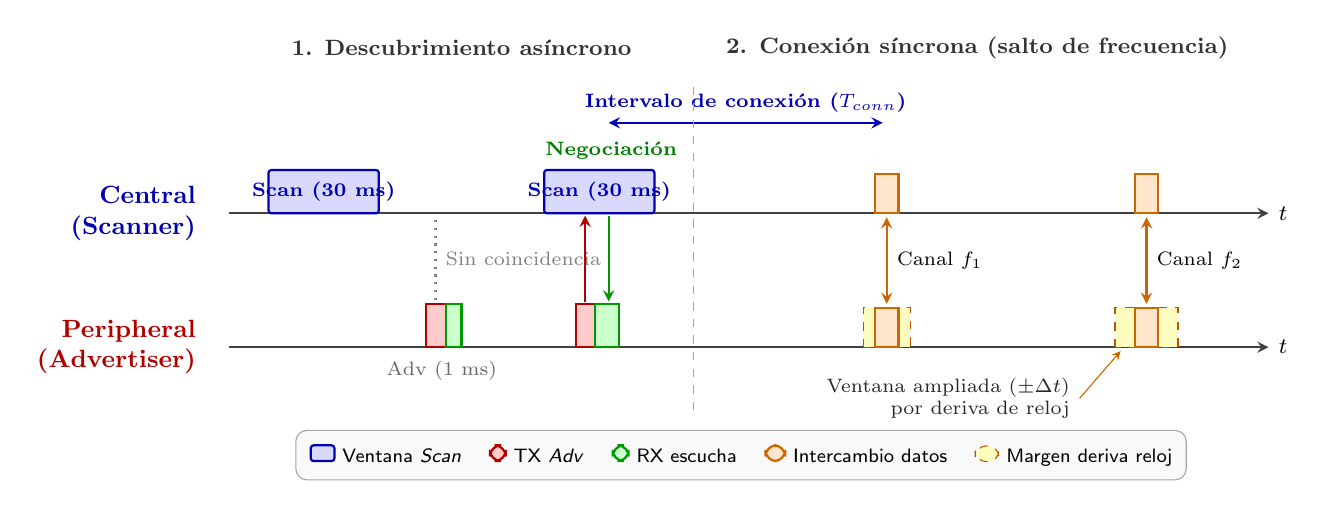
\begin{tikzpicture}[
                        font=\sffamily,
                        timeline/.style={->, >=stealth, thick, draw=black!75},
                        scan_win/.style={fill=blue!15, draw=blue!70!black, thick, rounded corners=1pt},
                        adv_tx/.style={fill=red!20, draw=red!70!black, thick},
                        adv_rx/.style={fill=green!20, draw=green!60!black, thick},
                        conn_pkt/.style={fill=orange!20, draw=orange!80!black, thick},
                        drift_win/.style={fill=yellow!25, draw=orange!70!black, dashed},
                        phase_box/.style={draw=gray!60, rounded corners=4pt, inner sep=6pt}
                    ]

                        % --- LABELS FOR THE TWO TIMELINES ---
                        \node[anchor=east, align=right, font=\small\bfseries, text=blue!70!black] (lbl_central) at (-0.3, 2.2) {Central\\(Scanner)};
                        \node[anchor=east, align=right, font=\small\bfseries, text=red!70!black] (lbl_periph) at (-0.3, 0.5) {Peripheral\\(Advertiser)};

                        % --- TIMELINE AXES ---
                        \draw[timeline] (0, 2.2) -- (13.2, 2.2) node[right, font=\footnotesize] {$t$};
                        \draw[timeline] (0, 0.5) -- (13.2, 0.5) node[right, font=\footnotesize] {$t$};

                        % =========================================================
                        % PHASE 1: ASYNCHRONOUS DISCOVERY (NO OVERLAP -> OVERLAP)
                        % =========================================================
                        % Cycle 1: Miss
                        \filldraw[scan_win] (0.5, 2.2) rectangle (1.9, 2.75) node[midway, font=\scriptsize\bfseries, text=blue!70!black] {Scan (30 ms)};
                        \filldraw[adv_tx] (2.5, 0.5) rectangle (2.75, 1.05);
                        \filldraw[adv_rx] (2.75, 0.5) rectangle (2.95, 1.05);
                        \node[below, font=\scriptsize, text=gray!80!black] at (2.7, 0.45) {Adv (1 ms)};
                        
                        % Dashed miss indicator
                        \draw[dotted, thick, gray] (2.62, 1.1) -- (2.62, 2.15) node[midway, right, font=\scriptsize, text=gray] {Sin coincidencia};

                        % Cycle 2: Hit!
                        \filldraw[scan_win] (4.0, 2.2) rectangle (5.4, 2.75) node[midway, font=\scriptsize\bfseries, text=blue!70!black] {Scan (30 ms)};
                        \filldraw[adv_tx] (4.4, 0.5) rectangle (4.65, 1.05);
                        \filldraw[adv_rx] (4.65, 0.5) rectangle (4.95, 1.05);

                        % Handshake arrows (Adv -> Scan -> CONNECT_IND)
                        \draw[->, >=stealth, thick, red!70!black] (4.52, 1.08) -- (4.52, 2.17);
                        \draw[->, >=stealth, thick, green!60!black] (4.82, 2.17) -- (4.82, 1.08);
                        \node[above, font=\scriptsize\bfseries, text=green!50!black, fill=white, inner sep=1pt] at (4.85, 2.85) {Negociación};

                        % =========================================================
                        % PHASE 2: SYNCHRONOUS CONNECTION EVENTS + CLOCK DRIFT
                        % =========================================================
                        % Connection Interval Bracket
                        \draw[<->, >=stealth, thick, blue!70!black] (4.82, 3.35) -- (8.3, 3.35)
                            node[midway, above, font=\scriptsize\bfseries, text=blue!70!black] {Intervalo de conexión ($T_{\text{conn}}$)};

                        % Event 1 (Ch X)
                        \filldraw[conn_pkt] (8.2, 2.2) rectangle (8.5, 2.7);
                        \filldraw[drift_win] (8.05, 0.5) rectangle (8.65, 1.0); % Window widening
                        \filldraw[conn_pkt] (8.2, 0.5) rectangle (8.5, 1.0);
                        \draw[<->, >=stealth, thick, orange!80!black] (8.35, 1.05) -- (8.35, 2.15)
                            node[midway, right, font=\scriptsize, text=black] {Canal $f_1$};

                        % Event 2 (Ch Y) - Showing Drift Widening
                        \filldraw[conn_pkt] (11.5, 2.2) rectangle (11.8, 2.7);
                        \filldraw[drift_win] (11.25, 0.5) rectangle (12.05, 1.0); % Wider window due to drift
                        \filldraw[conn_pkt] (11.5, 0.5) rectangle (11.8, 1.0);
                        \draw[<->, >=stealth, thick, orange!80!black] (11.65, 1.05) -- (11.65, 2.15)
                            node[midway, right, font=\scriptsize, text=black] {Canal $f_2$};

                        % Drift callout
                        \draw[<-, >=stealth, thin, orange!80!black] (11.32, 0.45) -- (10.8, -0.15)
                            node[left, align=right, font=\scriptsize, text=black!85] {Ventana ampliada ($\pm\Delta t$)\\por deriva de reloj};

                        % =========================================================
                        % PHASE DIVIDERS & HEADERS
                        % =========================================================
                        \draw[dashed, gray!70] (5.9, -0.3) -- (5.9, 3.8);
                        \node[font=\footnotesize\bfseries, text=black!80] at (2.95, 4.3) {1. Descubrimiento asíncrono};
                        \node[font=\footnotesize\bfseries, text=black!80] at (9.5, 4.3) {2. Conexión síncrona (salto de frecuencia)};

                        % =========================================================
                        % LEGEND
                        % =========================================================
                        \node[draw=gray!70, rounded corners, fill=gray!5, inner sep=5pt, anchor=north] at (6.5, -0.55) {
                            \scriptsize
                            \tikz \filldraw[scan_win] (0,0) rectangle (0.3,0.2); Ventana \emph{Scan} \quad
                            \tikz \filldraw[adv_tx] (0,0) rectangle (0.2,0.2); TX \emph{Adv} \quad
                            \tikz \filldraw[adv_rx] (0,0) rectangle (0.2,0.2); RX escucha \quad
                            \tikz \filldraw[conn_pkt] (0,0) rectangle (0.25,0.2); Intercambio datos \quad
                            \tikz \filldraw[drift_win] (0,0) rectangle (0.3,0.2); Margen deriva reloj
                        };

                    \end{tikzpicture}
                    \caption{Proceso de descubrimiento, negociación de conexión y sincronización periódica en BLE.}
                    \label{fig:ble_sync}
                \end{figure}


                El bajo consumo reside en que las activaciones son extremedamente cortas comparadas con los tiempos de sueño. Dado que las activaciones, de por sí, ya consumen poco (alrededor de miliamperios) se consigue un consumo medio de unos pocos microamperios, suficiente para duraciones de baterías de años.

                \paragraph{Comunicación sin conexión: Beacons}
                    Para aplicaciones que solo requieren difundir información periódica sin establecer un enlace bidireccional, BLE define el rol de \emph{Broadcaster} (emisor) y \emph{Observer} (receptor). Los dispositivos conocidos como \textbf{beacons} (balizas) aprovechan este modo enviando paquetes no conectables a intervalos configurables.

                    Al eliminar la sobrecarga de negociación y mantenimiento de una conexión, un beacon puede funcionar durante años con una única pila de botón (e.g., CR2032).

            \subsubsection{Perfil GATT y Características}
                A nivel de aplicación, BLE estructura los datos transmitidos mediante el perfil \textbf{GATT} (\emph{Generic Attribute Profile}), organizado jerárquicamente:

                \begin{itemize}
                    \item \textbf{Perfil (\emph{Profile}):} Agrupación funcional de servicios para un caso de uso concreto (e.g., monitorización cardíaca o sensor ambiental).
                    \item \textbf{Servicio (\emph{Service}):} Conjunto lógico de datos relacionados, identificado por un código único o \textbf{UUID}.
                    \item \textbf{Característica (\emph{Characteristic}):} Es la unidad mínima de datos en BLE. Cada característica encapsula un valor (e.g., temperatura actual), metadatos o descriptores (como unidades de medida) y permisos de acceso:
                    \begin{itemize}
                        \item \texttt{Read} / \texttt{Write}: El cliente solicita leer o modificar el valor de la característica bajo demanda.
                        \item \texttt{Notify} / \texttt{Indicate}: El periférico envía automáticamente el nuevo valor al cliente cada vez que cambia (con confirmación en el caso de \texttt{Indicate}), evitando el sondeo continuo (\emph{polling}) y ahorrando energía.
                    \end{itemize}
                    Las características tienen también un \textbf{UUID} identificador.
                \end{itemize}

                En esencia, un dispositivo anuncia mediante características los valores o variables a compartir, y el dispositivo remoto puede pedir lecturas, escrituras, notificaciones o indicaciones para interactuar con dichos valores.

        \subsection{Wi-Fi (IEEE 802.11)}

            Su objetivo principal es ofrecer un elevado ancho de banda y conectividad directa a redes IP, sobre las que se montará cualquier protocolo de comunicación siguiendo la arquitectura en capas de TCP/IP. Aunque tradicionalmente se ha descartado para nodos alimentados por baterías pequeñas, las variantes modernas y los modos de ahorro energético permiten su uso en determinados sistemas empotrados.

            \subsubsection{Capa física y acceso al medio}
                Wi-Fi opera principalmente en las bandas de 2.4 y 5GHz (y más recientemente en 6GHz con Wi-Fi 6E/7). Las diferentes versiones añaden cada vez más canales (y más anchos) para permitir mayores velocidades de transmisión de datos. Si bien, en las versiones de alta frecuencia, debido precisamente a la naturaleza de ellas, el rango se ve afectado negativamente.

                Para compartir el canal entre múltiples dispositivos sin que las transmisiones colisionen, Wi-Fi emplea el protocolo de acceso al medio \textbf{CSMA/CA} (\emph{Carrier Sense Multiple Access with Collision Avoidance}). Antes de emitir un paquete, el transceptor debe escuchar el canal para comprobar que está libre y esperar un tiempo aleatorio (\emph{backoff}). Esta escucha activa continua, sumada a modulaciones complejas, exige una potencia de transmisión y recepción significativamente mayor que en BLE (habitualmente decenas o cientos de miliamperios).

            \subsubsection{Conectividad y gestión del consumo energético}
                El punto de acceso o AP emite periódicamente tramas de baliza (\emph{Beacons}, típicamente cada 100ms) para anunciar la red y mantener sincronizados a los clientes. Para evitar que un dispositivo IoT tenga que mantener la antena encendida de forma ininterrumpida, el estándar incorpora mecanismos de ahorro de energía:

                \begin{itemize}
                    \item \textbf{Escucha periódica:} El nodo apaga su radio y se despierta únicamente cada cierto número de intervalos de baliza para escuchar una trama especial (\emph{DTIM}). En ella, el punto de acceso indica si tiene paquetes almacenados en búfer para ese nodo. Si no hay datos pendientes, el dispositivo vuelve a dormir inmediatamente.
                    \item \textbf{Target Wake Time (TWT):} Introducido en \textbf{Wi-Fi 6 (IEEE 802.11ax)}, permite que el nodo y el punto de acceso negocien horarios específicos y deterministas para despertarse e intercambiar datos, reduciendo tanto el tiempo de escucha activa como la contención en el canal (un enfoque conceptualmente similar a los eventos de conexión de BLE).
                \end{itemize}

                \begin{figure}[h]
                    \centering
                    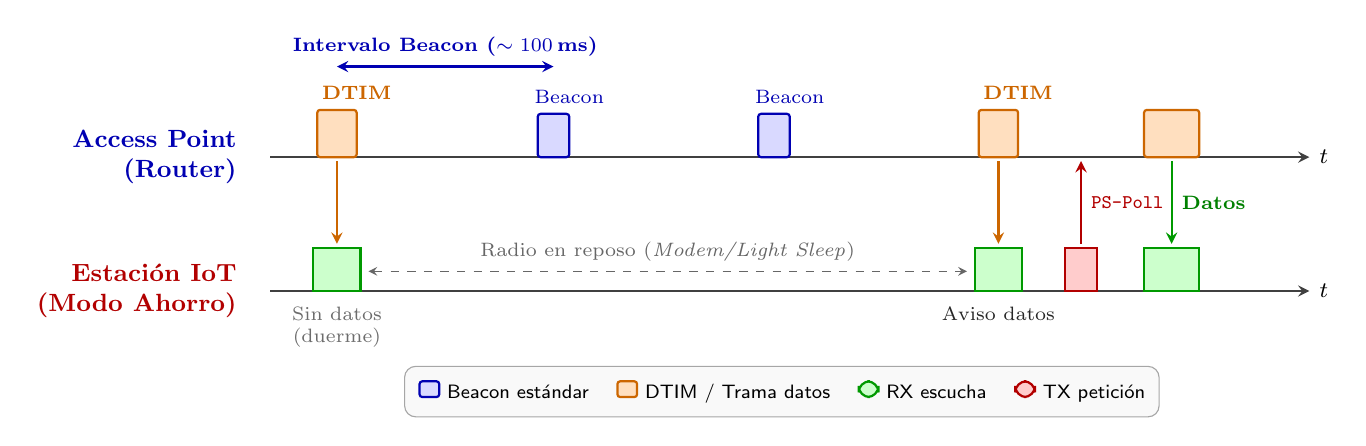
\begin{tikzpicture}[
                        font=\sffamily,
                        timeline/.style={->, >=stealth, thick, draw=black!75},
                        beacon/.style={fill=blue!15, draw=blue!70!black, thick, rounded corners=1pt},
                        dtim/.style={fill=orange!25, draw=orange!80!black, thick, rounded corners=1pt},
                        sta_rx/.style={fill=green!20, draw=green!60!black, thick},
                        sta_tx/.style={fill=red!20, draw=red!70!black, thick}
                    ]

                        % --- LABELS FOR THE TWO TIMELINES ---
                        \node[anchor=east, align=right, font=\small\bfseries, text=blue!70!black] at (-0.3, 2.2) {Access Point\\(Router)};
                        \node[anchor=east, align=right, font=\small\bfseries, text=red!70!black] at (-0.3, 0.5) {Estación IoT\\(Modo Ahorro)};

                        % --- TIMELINE AXES ---
                        \draw[timeline] (0, 2.2) -- (13.2, 2.2) node[right, font=\footnotesize] {$t$};
                        \draw[timeline] (0, 0.5) -- (13.2, 0.5) node[right, font=\footnotesize] {$t$};

                        % =========================================================
                        % AP BEACONS (Every ~2.8 units = 100 ms)
                        % =========================================================
                        % Beacon 1 (DTIM - No data)
                        \filldraw[dtim] (0.6, 2.2) rectangle (1.1, 2.8) node[above, font=\scriptsize\bfseries, text=orange!80!black] {DTIM};
                        
                        % Beacon 2 (Normal - STA sleeps)
                        \filldraw[beacon] (3.4, 2.2) rectangle (3.8, 2.75) node[above, font=\scriptsize, text=blue!70!black] {Beacon};

                        % Beacon 3 (Normal - STA sleeps)
                        \filldraw[beacon] (6.2, 2.2) rectangle (6.6, 2.75) node[above, font=\scriptsize, text=blue!70!black] {Beacon};

                        % Beacon 4 (DTIM - Data buffered!)
                        \filldraw[dtim] (9.0, 2.2) rectangle (9.5, 2.8) node[above, font=\scriptsize\bfseries, text=orange!80!black] {DTIM};

                        % Beacon Interval Bracket
                        \draw[<->, >=stealth, thick, blue!70!black] (0.85, 3.35) -- (3.6, 3.35)
                            node[midway, above, font=\scriptsize\bfseries, text=blue!70!black] {Intervalo Beacon ($\sim 100$\,ms)};

                        % =========================================================
                        % STATION ACTIVITY
                        % =========================================================
                        % Wake 1: Checks DTIM, buffer empty -> goes back to sleep
                        \filldraw[sta_rx] (0.55, 0.5) rectangle (1.15, 1.05);
                        \draw[->, >=stealth, thick, orange!80!black] (0.85, 2.15) -- (0.85, 1.1);
                        \node[below, align=center, font=\scriptsize, text=gray!85!black] at (0.85, 0.42) {Sin datos\\(duerme)};

                        % Sleep period annotation
                        \draw[<->, >=stealth, dashed, gray!80!black] (1.25, 0.75) -- (8.85, 0.75)
                            node[midway, above, font=\scriptsize, text=gray!80!black] {Radio en reposo (\emph{Modem/Light Sleep})};

                        % Wake 2: Checks DTIM, sees buffered data -> PS-Poll + Data RX
                        \filldraw[sta_rx] (8.95, 0.5) rectangle (9.55, 1.05);
                        \draw[->, >=stealth, thick, orange!80!black] (9.25, 2.15) -- (9.25, 1.1);
                        \node[below, align=center, font=\scriptsize, text=black!85] at (9.25, 0.42) {Aviso datos};

                        % Data exchange
                        \filldraw[sta_tx] (10.1, 0.5) rectangle (10.5, 1.05);
                        \draw[->, >=stealth, thick, red!70!black] (10.3, 1.1) -- (10.3, 2.15)
                            node[midway, right, font=\scriptsize, text=red!70!black] {\texttt{PS-Poll}};

                        \filldraw[dtim] (11.1, 2.2) rectangle (11.8, 2.8);
                        \filldraw[sta_rx] (11.1, 0.5) rectangle (11.8, 1.05);
                        \draw[->, >=stealth, thick, green!60!black] (11.45, 2.15) -- (11.45, 1.1)
                            node[midway, right, font=\scriptsize\bfseries, text=green!50!black] {Datos};

                        % =========================================================
                        % LEGEND
                        % =========================================================
                        \node[draw=gray!70, rounded corners, fill=gray!5, inner sep=5pt, anchor=north] at (6.5, -0.45) {
                            \scriptsize
                            \tikz \filldraw[beacon] (0,0) rectangle (0.25,0.2); Beacon estándar \quad
                            \tikz \filldraw[dtim] (0,0) rectangle (0.25,0.2); DTIM / Trama datos \quad
                            \tikz \filldraw[sta_rx] (0,0) rectangle (0.25,0.2); RX escucha \quad
                            \tikz \filldraw[sta_tx] (0,0) rectangle (0.25,0.2); TX petición
                        };

                    \end{tikzpicture}
                    \caption{Gestión del ahorro energético en Wi-Fi mediante escucha periódica de tramas \emph{DTIM}.}
                    \label{fig:wifi_psm}
                \end{figure}

                A pesar de estas optimizaciones, mantener la asociación con el punto de acceso y gestionar la pila de red completa implica que el consumo medio de un nodo Wi-Fi siga siendo superior al de BLE (habitualmente del orden de cientos de microamperios o pocos miliamperios). Por ello, suele reservarse para dispositivos conectados a la red eléctrica o con baterías recargables de cierta capacidad (cámaras IP, electrodomésticos o pasarelas). El beneficio principal es la mayor velocidad, ya que se pueden alcanzar las decenas de megabits por segundo con relativa facilidad.

            \subsubsection{Integración nativa con stack TCP/IP}
                Wi-Fi implementa únicamente las capas física y de enlace (niveles 1 y 2 del modelo OSI).

                Esto permite ejecutar de forma nativa el conjunto de protocolos estándar de Internet (\textbf{TCP/IP}):
                \begin{itemize}
                    \item \textbf{Direccionamiento y transporte directo:} Cada nodo obtiene una dirección IP (habitualmente mediante DHCP) y puede abrir conexiones TCP o UDP directamente contra servidores locales o en la nube.
                    \item \textbf{Compatibilidad directa con protocolos IoT:} Sobre esta pila de red se ejecutan sin necesidad de traducción protocolos de aplicación como \textbf{MQTT}, HTTP/REST o WebSockets, simplificando la arquitectura del sistema cuando la disponibilidad energética no es el factor limitante.
                \end{itemize}

        \subsection{LoRa y LoRaWAN}

            Muchas aplicaciones IoT en agricultura, entornos industriales o ciudades inteligentes requieren cubrir kilómetros con baterías que duren varios años. Para este escenario surgen las redes como \textbf{LoRa} en la capa física, complementado con \textbf{LoRaWAN} en las capas superiores. 

            \subsubsection{Capa física}
                \textbf{LoRa} (\emph{Long Range}) es una tecnología de modulación donde, en lugar de transmitir en una frecuencia fija, cada símbolo se codifica mediante un barrido continuo de frecuencia (\emph{chirp}) que aumenta o disminuye linealmente en el tiempo.

                Esta técnica proporciona una mayor sensibilidad en el receptor, permitiendo decodificar señales incluso por debajo del nivel de ruido ambiental y alcanzando distancias de entre \textbf{2 y 15\,km} en exteriores con muy baja potencia de emisión. LoRa opera en bandas alrededor de los \textbf{868\,MHz}, lo que mejora la penetración frente a obstáculos respecto a los 2.4\,GHz. La tasa de transferencia es, sin embargo, muy reducida (desde unos cientos de bits por segundo hasta unas pocas decenas de kbps). 
                
                Además, está sujeta a limitaciones legales de tiempo en el aire (\emph{duty cycle}, típicamente del 1\,\% en Europa), así como de uso de frecuencias (diferentes en cada parte del mundo).

            \subsubsection{Conectividad y bajo consumo (Clases de dispositivos)}
                Sobre la capa física LoRa se define el protocolo abierto \textbf{LoRaWAN}. Los nodos finales (\emph{End Devices}) emiten paquetes que son recogidos por uno o varios \emph{gateways} cercanos y reenviados mediante redes IP convencionales hacia un servidor de red central (\emph{Network Server}).

                LoRaWAN define tres clases de operación (para adaptarse a requisitos de latencia y consumo), siendo la \textbf{Clase A} la más habitual en nodos alimentados por batería:

                \begin{itemize}
                    \item \textbf{Clase A (Bidireccional asíncrona):} El nodo permanece en sueño profundo casi todo el tiempo y solo se despierta cuando tiene datos que enviar (\emph{uplink}). Inmediatamente después de transmitir, abre dos breves ventanas de recepción (\texttt{RX1} y \texttt{RX2}) para escuchar posibles mensajes de vuelta del servidor (\emph{downlink}). Si no recibe nada, vuelve a dormir. Es el modo de menor consumo, pero el servidor debe esperar a que el nodo transmita para poder comunicarse con él.
                    \item \textbf{Clase B (Ventanas programadas):} Además de las ventanas de Clase A, el nodo abre ventanas de recepción adicionales en instantes programados, sincronizándose mediante balizas periódicas (\emph{beacons}) emitidas por el \emph{gateway}.
                    \item \textbf{Clase C (Escucha continua):} Mantiene el receptor encendido de forma permanente excepto cuando transmite, ofreciendo latencia mínima para elementos conectados a la red eléctrica.
                \end{itemize}

                \begin{figure}[h]
                    \centering
                    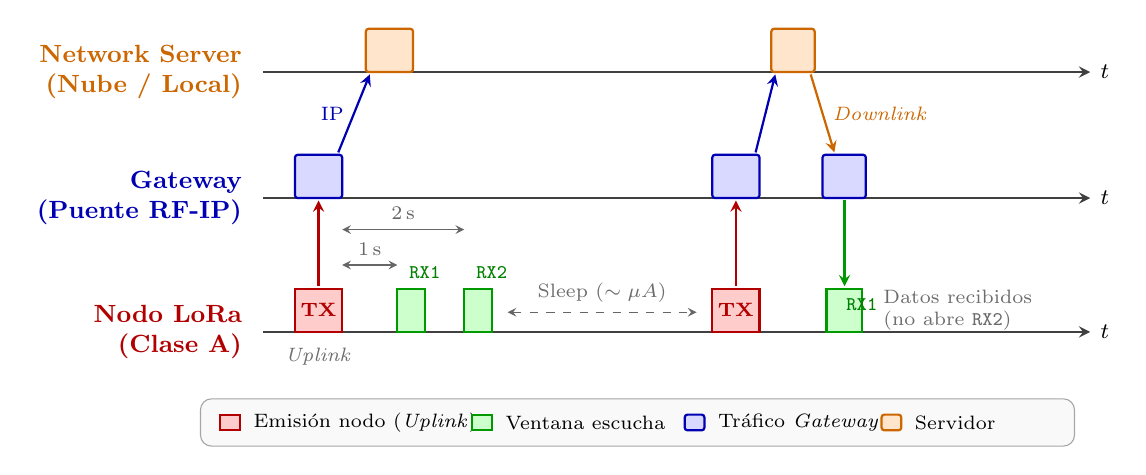
\begin{tikzpicture}[
                        font=\sffamily,
                        timeline/.style={->, >=stealth, thick, draw=black!75},
                        tx_pkt/.style={fill=red!20, draw=red!70!black, thick},
                        rx_win/.style={fill=green!20, draw=green!60!black, thick},
                        gw_pkt/.style={fill=blue!15, draw=blue!70!black, thick, rounded corners=1pt},
                        srv_pkt/.style={fill=orange!20, draw=orange!80!black, thick, rounded corners=1pt}
                    ]

                        % --- LABELS FOR THE TIMELINES ---
                        \node[anchor=east, align=right, font=\small\bfseries, text=red!70!black] at (-0.15, 0.5) {Nodo LoRa\\(Clase A)};
                        \node[anchor=east, align=right, font=\small\bfseries, text=blue!70!black] at (-0.15, 2.2) {Gateway\\(Puente RF-IP)};
                        \node[anchor=east, align=right, font=\small\bfseries, text=orange!80!black] at (-0.15, 3.8) {Network Server\\(Nube / Local)};

                        % --- TIMELINE AXES ---
                        \draw[timeline] (0, 0.5) -- (10.5, 0.5) node[right, font=\footnotesize] {$t$};
                        \draw[timeline] (0, 2.2) -- (10.5, 2.2) node[right, font=\footnotesize] {$t$};
                        \draw[timeline] (0, 3.8) -- (10.5, 3.8) node[right, font=\footnotesize] {$t$};

                        % =========================================================
                        % CYCLE 1: UPLINK ONLY (NO DOWNLINK AVAILABLE)
                        % =========================================================
                        % Node TX Uplink
                        \filldraw[tx_pkt] (0.4, 0.5) rectangle (1.0, 1.05) node[midway, font=\scriptsize\bfseries, text=red!70!black] {TX};
                        \node[below, font=\scriptsize, text=gray!85!black] at (0.7, 0.42) {\emph{Uplink}};

                        % Gateway receives and forwards via IP
                        \filldraw[gw_pkt] (0.4, 2.2) rectangle (1.0, 2.75);
                        \draw[->, >=stealth, thick, red!70!black] (0.7, 1.08) -- (0.7, 2.17);
                        
                        \filldraw[srv_pkt] (1.3, 3.8) rectangle (1.9, 4.35);
                        \draw[->, >=stealth, thick, blue!70!black] (0.95, 2.78) -- (1.35, 3.77) node[midway, left, font=\scriptsize, text=blue!70!black] {IP};

                        % RX1 and RX2 windows (empty)
                        \filldraw[rx_win] (1.7, 0.5) rectangle (2.05, 1.05) node[above, font=\scriptsize, text=green!50!black] {\texttt{RX1}};
                        \filldraw[rx_win] (2.55, 0.5) rectangle (2.9, 1.05) node[above, font=\scriptsize, text=green!50!black] {\texttt{RX2}};

                        % Delay brackets
                        \draw[<->, >=stealth, thin, gray!80!black] (1.0, 1.35) -- (1.7, 1.35) node[midway, above, font=\scriptsize] {1\,s};
                        \draw[<->, >=stealth, thin, gray!80!black] (1.0, 1.8) -- (2.55, 1.8) node[midway, above, font=\scriptsize] {2\,s};

                        % Deep sleep indicator
                        \draw[<->, >=stealth, dashed, gray!80!black] (3.1, 0.75) -- (5.5, 0.75)
                            node[midway, above, font=\scriptsize, text=gray!85!black] {Sleep ($\sim\mu\text{A}$)};

                        % =========================================================
                        % CYCLE 2: UPLINK + DOWNLINK RESPONSE IN RX1
                        % =========================================================
                        % Node TX Uplink
                        \filldraw[tx_pkt] (5.7, 0.5) rectangle (6.3, 1.05) node[midway, font=\scriptsize\bfseries, text=red!70!black] {TX};

                        % Gateway -> Server
                        \filldraw[gw_pkt] (5.7, 2.2) rectangle (6.3, 2.75);
                        \draw[->, >=stealth, thick, red!70!black] (6.0, 1.08) -- (6.0, 2.17);

                        \filldraw[srv_pkt] (6.45, 3.8) rectangle (7.0, 4.35);
                        \draw[->, >=stealth, thick, blue!70!black] (6.25, 2.78) -- (6.5, 3.77);

                        % Server schedules Downlink -> Gateway -> Node RX1
                        \filldraw[gw_pkt] (7.1, 2.2) rectangle (7.65, 2.75);
                        \draw[->, >=stealth, thick, orange!80!black] (6.95, 3.77) -- (7.25, 2.78) node[midway, right, font=\scriptsize, text=orange!80!black] {\emph{Downlink}};

                        \filldraw[rx_win] (7.15, 0.5) rectangle (7.6, 1.05) node[below, font=\scriptsize\bfseries, text=green!50!black] {\texttt{RX1}};
                        \draw[->, >=stealth, thick, green!60!black] (7.38, 2.17) -- (7.38, 1.08);

                        % RX2 skipped because RX1 succeeded
                        \node[right, align=left, font=\scriptsize, text=gray!85!black] at (7.75, 0.78) {Datos recibidos\\(no abre \texttt{RX2})};

                        % =========================================================
                        % LEGEND (Native TikZ shapes, no nested \tikz)
                        % =========================================================
                        \draw[gray!70, rounded corners, fill=gray!5] (-0.8, -0.95) rectangle (10.3, -0.35);
                        
                        \filldraw[tx_pkt] (-0.55, -0.75) rectangle (-0.3, -0.55);
                        \node[anchor=west, font=\scriptsize] at (-0.25, -0.65) {Emisión nodo (\emph{Uplink})};

                        \filldraw[rx_win] (2.65, -0.75) rectangle (2.9, -0.55);
                        \node[anchor=west, font=\scriptsize] at (2.95, -0.65) {Ventana escucha};

                        \filldraw[gw_pkt] (5.35, -0.75) rectangle (5.6, -0.55);
                        \node[anchor=west, font=\scriptsize] at (5.65, -0.65) {Tráfico \emph{Gateway}};

                        \filldraw[srv_pkt] (7.85, -0.75) rectangle (8.1, -0.55);
                        \node[anchor=west, font=\scriptsize] at (8.15, -0.65) {Servidor};

                    \end{tikzpicture}
                    \caption{Ciclo de transmisión y ventanas de recepción (\texttt{RX1}/\texttt{RX2}) en un nodo LoRaWAN de Clase A.}
                    \label{fig:lorawan_class_a}
                \end{figure}

            \subsubsection{Arquitectura de red y formato de datos}
                Los nodos LoRaWAN no implementan la pila TCP/IP ni disponen de una dirección IP propia, ya que la sobrecarga de sus cabeceras resultaría excesiva para enlaces de baja velocidad y paquetes pequeños (típicamente entre 11 y 242 bytes de carga útil según el factor de ensanchamiento).

                Para minimizar el tiempo en el aire, los sensores suelen enviar cargas útiles binarias muy compactas en bruto (\emph{raw bytes}) protegidas mediante cifrado de extremo a extremo (AES-128). Es el \emph{Network Server} (o servidor de aplicaciones) el encargado de decodificar estos bytes y reenviar la información ya estructurada hacia plataformas en la nube o brokers \textbf{MQTT}, actuando como puente entre la red LPWAN y los servicios IP estándar.

        \subsection{Zigbee}
            Mientras que Wi-Fi y BLE emplean habitualmente topologías en estrella (dependientes de un único punto de acceso o dispositivo central) y LoRaWAN apuesta por enlaces de largo alcance, \textbf{Zigbee} está diseñado para crear redes locales de sensores y actuadores de bajo consumo mediante \textbf{topologías en malla (\emph{mesh})}. Esto lo convierte en uno de los estándares más extendidos en domótica, donde no todos los dispositivos tienen por qué tener acceso a la red directamente, pero es casi seguro que se verán entre sí.

            \subsubsection{Capa física y de enlace (IEEE 802.15.4)}
                Zigbee no define su propia radio desde cero, sino que se construye sobre el estándar \textbf{IEEE 802.15.4}, el cual especifica las capas física (PHY) y de control de acceso al medio (MAC). Opera principalmente en la banda de frecuencia de los 2.4GHz, aunque puede usar otras (Como la de LoRa). Su tasa máxima de transferencia es de \textbf{250\,kbps}, suficiente para comandos de control y telemetría ligera.

            \subsubsection{Conectividad, roles y topología en malla}
                La principal característica de Zigbee es su capa de red, que permite que los dispositivos retransmitan paquetes de sus vecinos de forma automática y dinámica. Para gestionar el tráfico, la red distingue tres roles lógicos:

                \begin{itemize}
                    \item \textbf{Coordinador (\emph{Zigbee Coordinator}, ZC):} Existe uno único por red. Se encarga de inicializarla, seleccionar el canal y el identificador de red (\emph{PAN ID}), gestionar las claves de seguridad (AES-128) y actuar habitualmente como puente o \emph{gateway} hacia redes IP/MQTT.
                    \item \textbf{Enrutador (\emph{Zigbee Router}, ZR):} Nodos alimentados generalmente por la red eléctrica (como bombillas inteligentes o enchufes) que, además de ejecutar su propia función, mantienen la radio activa para encaminar mensajes de otros dispositivos y ampliar la cobertura espacial.
                    \item \textbf{Dispositivo Final (\emph{Zigbee End Device}, ZED):} Sensores o interruptores alimentados por batería. No enrutan tráfico ajeno, lo que les permite mantener su radio en sueño profundo casi todo el tiempo y despertarse únicamente para enviar datos o consultar periódicamente a su nodo padre (\emph{polling}).
                \end{itemize}

                \begin{figure}[h]
                    \centering
                    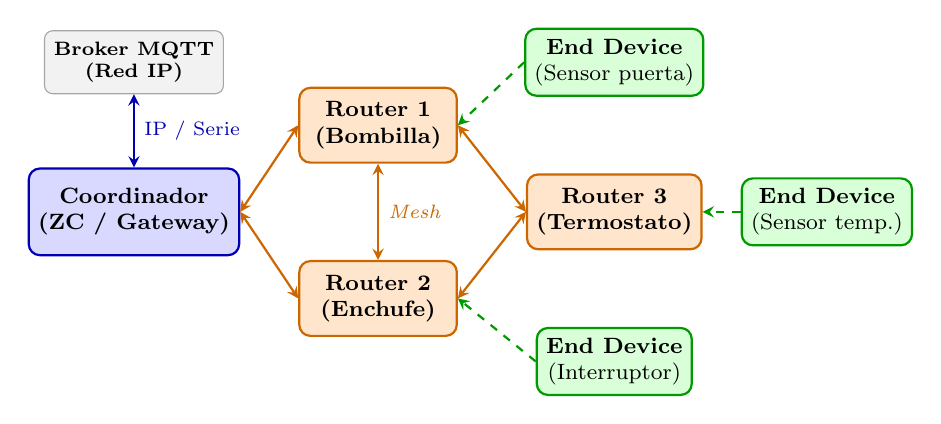
\begin{tikzpicture}[
                        font=\sffamily,
                        zc/.style={draw=blue!70!black, fill=blue!15, thick, rounded corners=4pt, minimum width=2.2cm, minimum height=1.1cm, align=center, font=\footnotesize\bfseries},
                        zr/.style={draw=orange!80!black, fill=orange!20, thick, rounded corners=4pt, minimum width=2.0cm, minimum height=0.95cm, align=center, font=\footnotesize\bfseries},
                        zed/.style={draw=green!60!black, fill=green!15, thick, rounded corners=4pt, minimum width=1.9cm, minimum height=0.85cm, align=center, font=\footnotesize},
                        mesh_link/.style={<->, >=stealth, thick, draw=orange!80!black},
                        zed_link/.style={->, >=stealth, thick, dashed, draw=green!60!black},
                        ip_link/.style={<->, >=stealth, thick, draw=blue!70!black}
                    ]

                        % --- NODES ---
                        % Coordinator & Gateway
                        \node[zc] (zc) at (1.5, 2.2) {Coordinador\\(ZC / Gateway)};
                        \node[draw=gray!70, fill=gray!10, rounded corners=3pt, minimum width=1.8cm, minimum height=0.8cm, align=center, font=\scriptsize\bfseries] (mqtt) at (1.5, 4.1) {Broker MQTT\\(Red IP)};

                        % Routers (Mains powered)
                        \node[zr] (zr1) at (4.6, 3.3) {Router 1\\(Bombilla)};
                        \node[zr] (zr2) at (4.6, 1.1) {Router 2\\(Enchufe)};
                        \node[zr] (zr3) at (7.6, 2.2) {Router 3\\(Termostato)};

                        % End Devices (Battery powered)
                        \node[zed] (zed1) at (7.6, 4.1) {\textbf{End Device}\\(Sensor puerta)};
                        \node[zed] (zed2) at (10.3, 2.2) {\textbf{End Device}\\(Sensor temp.)};
                        \node[zed] (zed3) at (7.6, 0.3) {\textbf{End Device}\\(Interruptor)};

                        % --- LINKS ---
                        % IP link
                        \draw[ip_link] (zc.north) -- (mqtt.south) node[midway, right, font=\scriptsize, text=blue!70!black] {IP / Serie};

                        % Mesh backbone links
                        \draw[mesh_link] (zc.east) -- (zr1.west);
                        \draw[mesh_link] (zc.east) -- (zr2.west);
                        \draw[mesh_link] (zr1.south) -- (zr2.north) node[midway, right, font=\scriptsize, text=orange!80!black] {\emph{Mesh}};
                        \draw[mesh_link] (zr1.east) -- (zr3.west);
                        \draw[mesh_link] (zr2.east) -- (zr3.west);

                        % End Device links (only to parent Router)
                        \draw[zed_link] (zed1.west) -- (zr1.east);
                        \draw[zed_link] (zed2.west) -- (zr3.east);
                        \draw[zed_link] (zed3.west) -- (zr2.east);

                    \end{tikzpicture}
                    \caption{Topología en malla (\emph{mesh}) de Zigbee y roles de los nodos hasta la pasarela MQTT.}
                    \label{fig:zigbee_mesh}
                \end{figure}

            \subsubsection{Modelo de datos y perfiles de aplicación}
                Zigbee define su propia capa de aplicación estandarizada mediante la \textbf{ZCL} (\emph{Zigbee Cluster Library}).

                En este modelo, cada dispositivo expone uno o varios \emph{endpoints} que agrupan funcionalidades llamadas \textbf{clústeres} (\emph{clusters}), equivalentes a los servicios en BLE. Cada clúster estandariza tanto los \textbf{atributos} (variables de estado, como el nivel de brillo o la temperatura) como los \textbf{comandos} (acciones como encender o apagar). Gracias a esta estandarización, dispositivos de distintos fabricantes pueden interoperar directamente, mientras que el Coordinador suele traducir estos clústeres hacia temas (\emph{topics}) de \textbf{MQTT} para su integración con plataformas de control centralizado.


        \subsection{Comunicación: el protocolo MQTT}
            Independientemente de la capa física subyacente, en numerosas ocasiones queremos que los datos acaben llegando a un servidor central en internet. Con WiFi es directo (ya que el nodo puede estar directamente conectado y conoce la pila TCP/IP). Con el resto de protocolos deberemos utilizar pasarlas hacia conectividad red estándar.

            Una vez ahí existen numerosos protocolos para la transferencia de datos de/hacia los nodos. Uno de los más extendidos, por su ligereza y versatilidad, es \textbf{MQTT}. \textbf{MQTT} es un protocolo para el intercambio de mensajes, diseñado para la comunicación en redes con ancho de banda limitado, y por dispositivos con capacidad de computación reducida. Adicionalmente, es transportable dentro de redes IP, por lo que se aprovecha de la conectividad general de internet. Debido a su simplicidad y escalabilidad, MQTT es de particular interés para aplicaciones de Internet de las cosas (IoT).

            MQTT utiliza un formato de mensaje binario (\Cref{fig:mqtt_packet}), que reduce enormemente la cantidad de información transmitida frente a otros protocolos basados en texto como \textbf{HTTP}.

            \begin{figure}[h]
                \centering
                \begin{tikzpicture}[
                    font=\sffamily,
                    box/.style={draw, rectangle, minimum height=1.1cm, align=center, inner sep=6pt, line width=0.8pt},
                    fh/.style={box, fill=blue!15, draw=blue!70!black},
                    vh/.style={box, fill=green!15, draw=green!70!black},
                    pl/.style={box, fill=orange!15, draw=orange!70!black},
                    subbox/.style={box, fill=blue!5, draw=blue!40!black, font=\sffamily\small}
                ]

                    % Level 1: Top-level Structure
                    \node[fh, minimum width=4.5cm] (fixed) {\textbf{Fixed Header}\\(2 to 5 Bytes)};
                    \node[vh, minimum width=3.5cm, right=0cm of fixed] (var) {\textbf{Variable Header}\\(Optional)};
                    \node[pl, minimum width=4.0cm, right=0cm of var] (payload) {\textbf{Payload}\\(Optional)};

                    \node[above=0.2cm of fixed.north west, anchor=south west, font=\sffamily\bfseries] {MQTT Control Packet Hierarchy};

                    % Level 2: Fixed Header Breakdown
                    \node[subbox, minimum width=6cm, anchor=north west] (byte1) at ($(fixed.south west) + (0,-1.2)$) {\textbf{Byte 1}\\Control Type \& Flags};
                    \node[subbox, minimum width=6cm, right=0cm of byte1] (byte2) {\textbf{Byte 2\dots Byte 5}\\Remaining Length (1--4 Bytes)};

                    \draw[thick, ->, >=stealth, blue!70!black] (fixed.south west) -- (byte1.north west);
                    \draw[thick, ->, >=stealth, blue!70!black] (fixed.south east) -- (byte2.north east);

                    % Level 3: Byte 1 Bit Breakdown
                    \node[subbox, fill=blue!25, minimum width=3cm, anchor=north west] (type) at ($(byte1.south west) + (0,-1.2)$) {\textbf{Bits 7--4}\\Packet Type (15 types)\\e.g., $0001_2$ = CONNECT};
                    \node[subbox, fill=blue!10, minimum width=3cm, right=0cm of type] (flags) {\textbf{Bits 3--0}\\Flags Specific to Type\\e.g., DUP, QoS, RETAIN};

                    \draw[thick, ->, >=stealth, blue!70!black] (byte1.south west) -- (type.north west);
                    \draw[thick, ->, >=stealth, blue!70!black] (byte1.south east) -- (flags.north east);

                \end{tikzpicture}
                \caption{Formato de los paquetes \textbf{MQTT}}
                \label{fig:mqtt_packet}
            \end{figure}

            En \textbf{MQTT} se distinguen los \emph{clientes} y los \emph{brokers}. Un cliente puede enviar mensajes al broker (conteniendo generalmente actualizaciones de valores etiquetados), y el broker reenvía estas actualizaciones a otros clientes que estén suscritos a dichos valores etiquetados. Las etiquetas se indican categorizadas, con cada categoría separada por ``/''. Así, se permiten suscripciones a categorías completas, por ejemplo. Un ejemplo sencillo de esta estructura puede verse en la \Cref{fig:mqtt_diagram}


            \begin{figure}[h]
                \centering
                \begin{tikzpicture}[
                    font=\sffamily,
                    % Define node styles
                    node_base/.style={draw, thick, rectangle, rounded corners, minimum height=1.5cm, align=center, inner sep=10pt},
                    broker/.style={node_base, fill=blue!10, draw=blue!70!black, minimum width=3cm, font=\sffamily\bfseries},
                    client/.style={node_base, fill=white, draw=gray, minimum width=2.5cm},
                    % Define arrow styles
                    arrow_style/.style={-{Stealth[scale=1.0]}, thick},
                    pub_arrow/.style={arrow_style, draw=red!70!black, densely dashed},
                    sub_arrow/.style={arrow_style, draw=green!60!black}
                ]

                    % --- 1. The MQTT Broker (The Core) ---
                    \node[broker] (broker) {
                        \textbf{MQTT Broker} \\
                        (e.g., ThingsBoard) 
                    };

                    % --- 2. Client that is ONLY a Publisher (Sensor) ---
                    \node[client, left=2.8cm of broker] (sensor) {
                        Temp. Sensor \\ (Kitchen) \\
                        \textbf{\textcolor{red!70!black}{Publisher}}
                    };

                    % --- 3. Client that is ONLY a Subscriber (Actuator) ---
                    \node[client, right=2.5cm of broker] (lock) {
                        Front Door Lock \\
                        \textbf{\textcolor{green!60!black}{Subscriber}}
                    };

                    % --- 4. Client that is BOTH (The Hub) ---
                    \node[client, above=2cm of broker] (hub) {
                        Smart Home Hub (Tablet) \\
                        \textbf{\textcolor{red!70!black}{Publisher}} \& \textbf{\textcolor{green!60!black}{Subscriber}}
                    };


                    % --- DRAWING INTERACTIONS AND FLOWS ---

                    % Flow Set A: Temperature Data (Sensor -> Broker -> Hub)
                    % Publish connection from sensor to broker
                    \draw[pub_arrow] (sensor.east) -- (broker.west) 
                        node[midway, above, text=red!70!black, font=\small\bfseries] {PUBLISH}
                        node[midway, below, font=\footnotesize] {\texttt{home/kitchen/temp}}
                        node[midway, below=0.4cm, font=\footnotesize, fill=white] {Payload: \texttt{22.5°C}};

                    % Subscribe connection from broker to hub
                    \draw[sub_arrow] (broker.north) .. controls +(0,1.2) and +(0,-1.2) .. (hub.south)
                        node[midway, right=0.3cm, text=green!60!black, font=\small\bfseries, anchor=west] {SUBSCRIBE}
                        node[midway, right=0.3cm, font=\footnotesize, anchor=west, yshift=-0.4cm] {\texttt{home/kitchen/temp}};

                        
                    % Flow Set B: Lock Command (Hub -> Broker -> Lock)
                    % Publish connection from hub back to broker
                    % Note: Using slightly different anchors to keep lines separated
                    \draw[pub_arrow] ($(hub.south)+(-0.3,0)$) .. controls +(-0.8,-1.2) and +(-0.8,1.2) .. ($(broker.north)+(-0.3,0)$)
                        node[pos=0.3, left=0.1cm, text=red!70!black, font=\small\bfseries, anchor=east] {PUBLISH}
                        node[pos=0.3, left=0.1cm, font=\footnotesize, anchor=east, yshift=-0.4cm] {\texttt{home/door/lock}}
                        node[pos=0.3, left=0.1cm, font=\footnotesize, anchor=east, yshift=-0.7cm] {Payload: \texttt{UNLOCK}};

                    % Subscribe connection from broker to lock
                    \draw[sub_arrow] (broker.east) -- (lock.west)
                        node[midway, above, text=green!60!black, font=\small\bfseries] {SUBSCRIBE}
                        node[midway, below, font=\footnotesize] {\texttt{home/door/lock}};


                    % --- LEGEND ---
                    \node[draw, thick, rounded corners, fill=white, inner sep=6pt, anchor=north, yshift=-1cm] (legend) at (broker.south) {
                        \begin{minipage}{5cm}
                        \small \textbf{Legend:} \\
                        \tikz \draw[pub_arrow] (0,0) -- (0.6,0); \textcolor{red!70!black}{ Publish Message (Out)} \\
                        \tikz \draw[sub_arrow] (0,0) -- (0.6,0); \textcolor{green!60!black}{ Subscribe Message (In)} \\
                        Note: Red/Green dotted lines represent MQTT control packets (not physical cables).
                        \end{minipage}
                    };
                \end{tikzpicture}
                \caption{Generic MQTT diagram}
                \label{fig:mqtt_diagram}
            \end{figure}

            \subsubsection{Transporte en MQTT}
                MQTT opera en la capa de aplicación sobre \textbf{TCP/IP} (habitualmente en el puerto 1883, o 8883 cuando se cifra mediante TLS). Gracias a TCP, MQTT hereda el control de flujo y la entrega ordenada de paquetes, añadiendo además sus propios mecanismos para adaptarse a enlaces inalámbricos inestables:

                \begin{itemize}
                    \item \emph{Quality of Service} o \textbf{QoS:} Permiten equilibrar fiabilidad y consumo de ancho de banda mensaje a mensaje:
                    \begin{itemize}
                        \item \textbf{QoS 0 (\emph{At most once}):} El mensaje se envía una única vez sin confirmación. Es el modo más rápido y ligero, ideal para lecturas periódicas de sensores donde perder una muestra puntual no importa.
                        \item \textbf{QoS 1 (\emph{At least once}):} Garantiza que el mensaje llega al receptor mediante un paquete de confirmación. Si no se recibe confirmación, el emisor retransmite el paquete, pudiendo generar duplicados.
                        \item \textbf{QoS 2 (\emph{Exactly once}):} Asegura que el mensaje se entrega exactamente una vez, evitando duplicados a costa de mayor latencia y tráfico de red.
                    \end{itemize}

                    \item \textbf{Formato del \emph{Payload}:} MQTT es completamente agnóstico al contenido de la carga útil. Aunque se puede emplear texto estructurado como \textbf{JSON}, en enlaces restringidos se transmiten tramas binarias compactas para minimizar el tamaño del paquete.
                \end{itemize}

            \subsubsection{Integración mediante pasarelas (\emph{Bridges} / \emph{Gateways})}
                Mientras que los dispositivos \textbf{Wi-Fi} o Ethernet implementan la pila TCP/IP completa y actúan directamente como clientes MQTT, las tecnologías como \textbf{BLE}, \textbf{Zigbee} o \textbf{LoRaWAN} carecen de direccionamiento IP nativo para ahorrar batería y ancho de banda.

                Para integrar estos nodos en una arquitectura centralizada se emplean pasarelas o (\emph{gateways}). Estos equipos disponen simultáneamente de interfaces radio de bajo consumo y conexión IP, actuando como traductores bidireccionales (\Cref{fig:mqtt_bridges}):

                \begin{enumerate}
                    \item La pasarela recoge los datos en el formato nativo de cada tecnología: notificaciones de características \textbf{GATT} o paquetes \emph{advertising} en BLE, atributos de clústeres \textbf{ZCL} en Zigbee, o tramas cifradas en bruto en LoRaWAN.
                    \item El \emph{gateway} traduce el identificador físico del dispositivo (dirección MAC, IEEE de 64 bits o \emph{DevEUI}) y el tipo de magnitud a una ruta estructurada de MQTT (por ejemplo, \texttt{zigbee2mqtt/sensor\_salon/temperatura} o \texttt{lorawan/finca1/nodo04/humedad}).
                    \item Los valores binarios se convierten habitualmente a un formato homogéneo (como JSON) y se publican en el broker. De forma simétrica, cuando una aplicación publica una orden en un \emph{topic} de control (e.g., \texttt{.../set}), la pasarela se suscribe a él, traduce el comando al protocolo radio correspondiente y lo envía al actuador, confirmando opcionalmente, si el protocolo lo permite, la recepción.
                \end{enumerate}

                \begin{figure}[h]
                    \centering
                    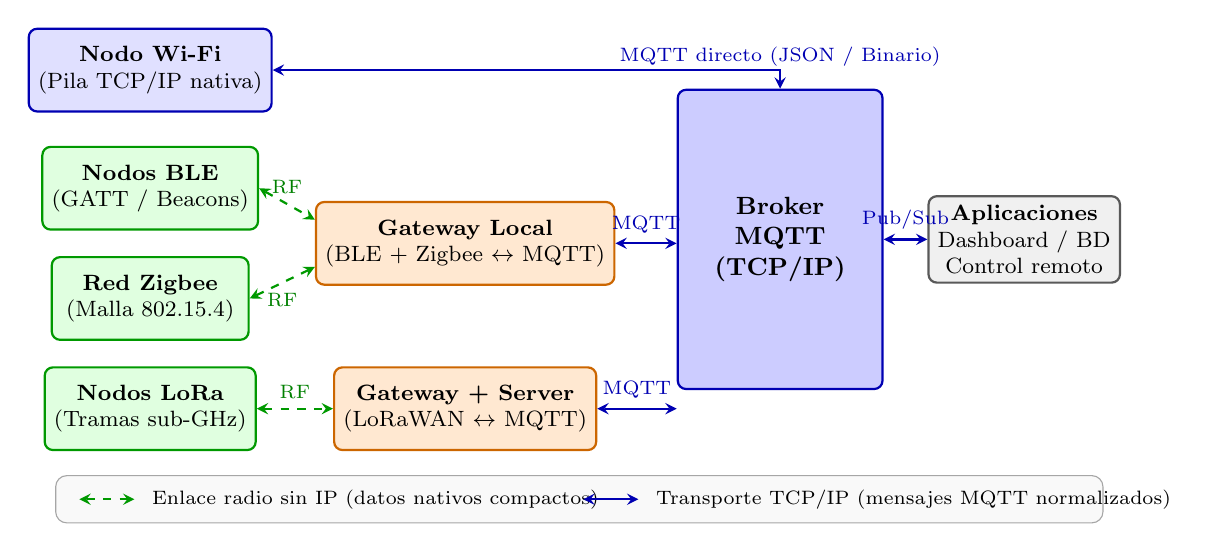
\begin{tikzpicture}[
                        font=\sffamily,
                        node_box/.style={draw, thick, rounded corners=3pt, minimum height=1.05cm, align=center, font=\footnotesize},
                        radio_node/.style={node_box, fill=green!12, draw=green!60!black, minimum width=2.5cm},
                        wifi_node/.style={node_box, fill=blue!12, draw=blue!70!black, minimum width=2.5cm},
                        gw_box/.style={node_box, fill=orange!18, draw=orange!80!black, minimum width=2.6cm},
                        broker_box/.style={node_box, fill=blue!20, draw=blue!70!black, minimum width=2.6cm, minimum height=3.8cm, font=\small\bfseries},
                        app_box/.style={node_box, fill=gray!12, draw=gray!70!black, minimum width=2.2cm},
                        flow_rf/.style={<->, >=stealth, thick, dashed, draw=green!60!black},
                        flow_ip/.style={<->, >=stealth, thick, draw=blue!70!black}
                    ]

                        % --- LEFT COLUMN: END DEVICES ---
                        \node[wifi_node] (wifi) at (1.3, 4.2) {\textbf{Nodo Wi-Fi}\\(Pila TCP/IP nativa)};
                        \node[radio_node] (ble) at (1.3, 2.7) {\textbf{Nodos BLE}\\(GATT / Beacons)};
                        \node[radio_node] (zig) at (1.3, 1.3) {\textbf{Red Zigbee}\\(Malla 802.15.4)};
                        \node[radio_node] (lora) at (1.3, -0.1) {\textbf{Nodos LoRa}\\(Tramas sub-GHz)};

                        % --- MIDDLE COLUMN: GATEWAYS / BRIDGES ---
                        \node[gw_box] (gw_local) at (5.3, 2.0) {\textbf{Gateway Local}\\(BLE + Zigbee $\leftrightarrow$ MQTT)};
                        \node[gw_box] (gw_lora) at (5.3, -0.1) {\textbf{Gateway + Server}\\(LoRaWAN $\leftrightarrow$ MQTT)};

                        % --- RIGHT COLUMN: BROKER & CONSUMERS ---
                        \node[broker_box] (broker) at (9.3, 2.05) {Broker\\MQTT\\(TCP/IP)};
                        \node[app_box] (app) at (12.4, 2.05) {\textbf{Aplicaciones}\\Dashboard / BD\\Control remoto};

                        % --- CONNECTIONS ---
                        % Wi-Fi direct to Broker
                        \draw[flow_ip] (wifi.east) -- (9.3, 4.2) -- (broker.north)
                            node[pos=0.35, above, font=\scriptsize, text=blue!70!black] {MQTT directo (JSON / Binario)};

                        % BLE & Zigbee to Local Gateway
                        \draw[flow_rf] (ble.east) -- (gw_local.west |- 0,2.3) node[midway, above, font=\scriptsize, text=green!50!black] {RF};
                        \draw[flow_rf] (zig.east) -- (gw_local.west |- 0,1.7) node[midway, below, font=\scriptsize, text=green!50!black] {RF};

                        % Local Gateway to Broker
                        \draw[flow_ip] (gw_local.east) -- (broker.west |- 0,2.0)
                            node[midway, above, font=\scriptsize, text=blue!70!black] {MQTT};

                        % LoRa to LoRa Gateway/Server
                        \draw[flow_rf] (lora.east) -- (gw_lora.west) node[midway, above, font=\scriptsize, text=green!50!black] {RF};

                        % LoRa Server to Broker
                        \draw[flow_ip] (gw_lora.east) -- (broker.west |- 0,-0.1)
                            node[midway, above, font=\scriptsize, text=blue!70!black] {MQTT};

                        % Broker to Applications
                        \draw[flow_ip] (broker.east) -- (app.west)
                            node[midway, above, font=\scriptsize, text=blue!70!black] {Pub/Sub};

                        % --- LEGEND ---
                        \draw[gray!70, rounded corners, fill=gray!5] (0.1, -1.55) rectangle (13.4, -0.95);

                        \draw[flow_rf] (0.4, -1.25) -- (1.1, -1.25);
                        \node[anchor=west, font=\scriptsize] at (1.2, -1.25) {Enlace radio sin IP (datos nativos compactos)};

                        \draw[flow_ip] (6.8, -1.25) -- (7.5, -1.25);
                        \node[anchor=west, font=\scriptsize] at (7.6, -1.25) {Transporte TCP/IP (mensajes MQTT normalizados)};

                    \end{tikzpicture}
                    \caption{Arquitectura de integración en MQTT: conexión nativa sobre IP frente a pasarelas (\emph{bridges}) para tecnologías de bajo consumo.}
                    \label{fig:mqtt_bridges}
                \end{figure}

                Uno de los principales usos finales de todos estos sistemas es la integración con Dashboards, que permiten visualizar todos los nodos conectados, ver sus características y valores, así como mandar comandos para actualizarlos.

        \subsection{Actualizaciones remotas}
            Hemos visto ya cómo se pueden enviar o recibir datos. ¿Pero, y qué hay de las actualizaciones de Firmware/Software? Especialmente en dispositivos IoT, es interesante, una vez desplegado un sistema, tener la capacidad de corregir vulnerabilidades de seguridad, solucionar errores o añadir nuevas funcionalidades sin intervención física. Existen distintas estrategias para actualizar el \emph{firmware} de un dispositivo IoT:

            \subsubsection{Métodos de actualización de firmware}
                Según el acceso físico al dispositivo y la infraestructura disponible, las actualizaciones se clasifican en tres grandes grupos:

                \begin{itemize}
                    \item \textbf{Programación directa mediante interfaz hardware (JTAG / SWD / UART):} Es el método habitual durante las fases de desarrollo y fabricación. Requiere conectar un programador físico a los pines de depuración del microcontrolador para escribir directamente en la memoria \emph{flash}. Aunque ofrece control total (incluso sobre un sistema bloqueado), es inviable en despliegues masivos o ubicaciones remotas.
                    \item \textbf{Actualización local mediante almacenamiento externo o enlace cercano:} El usuario o técnico interviene localmente mediante una tarjeta SD, una memoria USB o una conexión inalámbrica de corto alcance (por ejemplo, \textbf{BLE DFU}, \emph{Device Firmware Update}) utilizando un teléfono móvil como puente para transferir el binario.
                    \item \textbf{Actualización inalámbrica remota (\emph{Over-The-Air}, OTA):} El dispositivo descarga el nuevo binario de forma autónoma a través de la red (habitualmente mediante Wi-Fi, 5G, o a través de una pasarela en redes Zigbee/LoRa/BLE), valida su integridad y se reprograma a sí mismo sin asistencia humana.
                \end{itemize}

            \subsubsection{Arquitectura de una actualización OTA y particionado A/B}
                El mayor riesgo de una actualización remota es que un corte de suministro eléctrico o una pérdida de conexión deje la memoria de programa corrupta, inutilizando el dispositivo de forma permanente.

                Para evitarlo, los sistemas empotrados modernos dividen su memoria \emph{flash} no volátil en dos particiones gestionadas por un gestor de arranque (\textbf{\emph{bootloader}}), empleando un esquema dual A/B:

                \begin{enumerate}
                    \item Mientras el sistema sigue ejecutando su versión estable desde la partición activa (\texttt{OTA\_0}), el código de aplicación descarga el nuevo binario y lo escribe en la partición inactiva (\texttt{OTA\_1}).
                    \item Antes de aplicar el cambio, el dispositivo comprueba la integridad del binario mediante una suma de verificación (SHA-256) y valida su autenticidad mediante firma digital, impidiendo la ejecución de código malicioso o corrupto.
                    \item El \emph{bootloader} marca la partición \texttt{OTA\_1} como pendiente de prueba y reinicia el microcontrolador. Si el nuevo \emph{firmware} arranca correctamente y confirma su estado operativo (por ejemplo, reconectándose al servidor), la partición pasa a ser definitiva. Si falla o se reinicia inesperadamente, el \emph{bootloader} revierte automáticamente a la partición anterior (\texttt{OTA\_0}).
                \end{enumerate}

                \begin{figure}[h]
                    \centering
                    \begin{tikzpicture}[
                        font=\sffamily,
                        % Fixed width and height so every partition aligns identically
                        mem_box/.style={
                            draw, thick,
                            minimum width=2.7cm, text width=2.5cm,
                            minimum height=0.95cm,
                            align=center, font=\scriptsize, inner sep=3pt
                        },
                        boot/.style={mem_box, fill=gray!20, draw=gray!80!black},
                        active/.style={mem_box, fill=green!18, draw=green!60!black},
                        inactive/.style={mem_box, fill=blue!12, draw=blue!70!black},
                        downloading/.style={mem_box, fill=orange!20, draw=orange!80!black},
                        nvs/.style={mem_box, fill=yellow!20, draw=orange!60!black, minimum height=0.6cm},
                        step_arrow/.style={->, >=stealth, thick, draw=black!75}
                    ]

                        % =========================================================
                        % STEP 1: NORMAL OPERATION + DOWNLOAD
                        % =========================================================
                        \node[font=\footnotesize\bfseries, text=black!85] (t1) at (1.4, 4.4) {1. Descarga en \texttt{OTA\_1}};
                        \node[boot] (b1) at (1.4, 3.55) {\textbf{Bootloader}};
                        \node[active, below=0pt of b1] (a1) {\textbf{Partición A (\texttt{OTA\_0})}\\Firmware v1.0 (Activo)};
                        \node[downloading, below=0pt of a1] (p1) {\textbf{Partición B (\texttt{OTA\_1})}\\Recibiendo\\v1.1...};
                        \node[nvs, below=0pt of p1] (n1) {Datos / Config (NVS)};

                        % Cloud download arrow (routed cleanly to the left of NVS)
                        \node[draw=blue!70!black, fill=blue!10, rounded corners=3pt, font=\scriptsize\bfseries, align=center, inner sep=4pt, below=0.55cm of n1] (srv) {Servidor HTTP / MQTT\\(Binario v1.1 firmado)};
                        \draw[->, >=stealth, thick, orange!80!black] (srv.west) -- ++(-0.35, 0) |- (p1.west)
                            node[pos=0.25, left, font=\scriptsize, text=orange!80!black] {TLS};

                        % =========================================================
                        % STEP 2: VERIFICATION & REBOOT
                        % =========================================================
                        \node[font=\footnotesize\bfseries, text=black!85] (t2) at (5.7, 4.4) {2. Verificación y Reinicio};
                        \node[boot] (b2) at (5.7, 3.55) {\textbf{Bootloader}};e) --
                        \node[inactive, below=0pt of b2] (a2) {\textbf{Partición A (\texttt{OTA\_0})}\\Firmware v1.0 (Respaldo)};
                        \node[downloading, below=0pt of a2] (p2) {\textbf{Partición B (\texttt{OTA\_1})}\\v1.1 Verificado (Prueba)};
                        \node[nvs, below=0pt of p2] (n2) {Datos / Config (NVS)};

                        % =========================================================
                        % STEP 3: CONFIRMED OR ROLLBACK
                        % =========================================================
                        \node[font=\footnotesize\bfseries, text=black!85] (t3) at (10.0, 4.4) {3. Confirmación o Fallo};
                        \node[boot] (b3) at (10.0, 3.55) {\textbf{Bootloader}};
                        \node[inactive, below=0pt of b3] (a3) {\textbf{Partición A (\texttt{OTA\_0})}\\v1.0 (Lista para futura OTA)};
                        \node[active, below=0pt of a3] (p3) {\textbf{Partición B (\texttt{OTA\_1})}\\Firmware v1.1 (Activo)};
                        \node[nvs, below=0pt of p3] (n3) {Datos / Config (NVS)};

                        % =========================================================
                        % TRANSITION ARROWS & ROLLBACK
                        % =========================================================
                        \draw[step_arrow] (a1.east) -- (p2.west)
                            node[midway, above, font=\scriptsize] {Reinicio};

                        \draw[step_arrow] (p2.east) -- (p3.west)
                            node[midway, above, font=\scriptsize, text=green!50!black] {OK};

                        % Rollback curved arrow below Step 2 -> back to Partition A
                        \draw[->, >=stealth, thick, dashed, red!70!black] (p2.east) -| ++(0.3, -1.85) -| ([xshift=-0.35cm]a2.west) -- (a2.west);
                        \node[font=\scriptsize, text=red!70!black, align=center] at (5.7, -1.35) {Si falla el arranque:\\\emph{Rollback} a Partición A};

                    \end{tikzpicture}
                    \caption{Esquema de memoria \emph{flash} dual (A/B) durante una actualización OTA segura con recuperación ante fallos.}
                    \label{fig:ota_partitions}
                \end{figure}

            \subsubsection{Transporte de actualizaciones}
                La forma de transmisión del nuevo \emph{firmware} varía según el ancho de banda y la arquitectura del protocolo utilizado:

                \begin{itemize}
                    \item Aun en redes de alta velocidad (e.g: MQTT sobre WiFi), transferir archivos binarios grandes directamente a través del broker puede saturar la red. La práctica estándar consiste en notificar la disponibilidad de la actualización mediante un mensaje ligero en MQTT (incluyendo la URL de descarga, la versión y el \emph{hash} esperado) para que el dispositivo descargue el archivo mediante \textbf{HTTPS} en bloques fragmentados.
                    
                    \item En enlaces lentos o con ciclos de trabajo muy limitados, enviar cientos de kilobytes puede llevar desde varios minutos (en Zigbee o BLE) hasta horas o días (en LoRaWAN). En estos casos se recurre a actualizaciones diferenciales, transmitiendo únicamente las diferencias binarias respecto a la versión anterior hasta que se recibe la actualización completa.
                \end{itemize}

\end{document}